\documentclass[10pt]{article}
    \usepackage[top=2cm,bottom=3cm,left=2cm,right=2cm]{geometry}

    % amsmath and amssymb packages, useful for mathematical formulas and symbols
    \usepackage{amsmath,amssymb}

    % Use Unicode characters when possible
    \usepackage[utf8]{inputenc}

    % textcomp package and marvosym package for additional characters
    \usepackage{textcomp,marvosym}

    % cite package, to clean up citations in the main text. Do not remove.
    \usepackage{cite}

    % Use nameref to cite supporting information files (see Supporting Information section for more info)
    \usepackage{nameref,hyperref}

    % line numbers
    \usepackage[right]{lineno}

    % ligatures disabled
    \usepackage{microtype}
    \DisableLigatures[f]{encoding = *, family = * }

    % color can be used to apply background shading to table cells only
    \usepackage[table]{xcolor}

    % array package and thick rules for tables
    \usepackage{array}

    \usepackage{tikz}
    \usetikzlibrary{calc}

\newcommand\samplesTikz{10}
\def\Spline#1#2#3#4#5#6#7#8{%Px Py Qx Qy px py qx qy
    plot (
        {   (#1) + (#5)*(\t) + (3*(#3) - 3*(#1) - 2*(#5) - (#7))*(\t)*(\t) + (2*(#1) - 2*(#3) + (#5) + (#7))*(\t)*(\t)*(\t)   },
        {   (#2) + (#6)*(\t) + (3*(#4) - 3*(#2) - 2*(#6) - (#8))*(\t)*(\t) + (2*(#2) - 2*(#4) + (#6) + (#8))*(\t)*(\t)*(\t)   }
    )
}
% \def\ESpline#1#2#3#4#5#6#7#8{%Px Py Qx Qy px py qx qy
%     plot (
%         {   (#1) + (#5)*(\t) + (3*(#3) - 3*(#1) - 2*(#5) - (#7))*(\t)*(\t) + (2*(#1) - 2*(#3) + (#5) + (#7))*(\t)*(\t)*(\t)   },
%         {   (#2) + (#6)*(\t) + (3*(#4) - 3*(#2) - 2*(#6) - (#8))*(\t)*(\t) + (2*(#2) - 2*(#4) + (#6) + (#8))*(\t)*(\t)*(\t)   }
%     )
% }

\DeclareMathOperator{\cis}{cis}
\DeclareMathOperator{\acos}{acos}
\DeclareMathOperator{\Lspline}{L}
\DeclareMathOperator{\nLspline}{nL}
\DeclareMathOperator{\Espline}{E}
\DeclareMathOperator{\Fspline}{F}
% for the drawing of examples taken from the c++ coded version. neccessary because TikZ constrols work different than the formulae of the Splines, I use
\newcommand\controlfactor{.32}

\title{Theory on Vi Hart's Flippy Chips}
\author{Anton Obersteiner}

\begin{document}
\maketitle

\begin{figure}[h]
    \begin{tikzpicture}[scale=8]
        \node[inner sep=0pt, outer sep=0pt] (A) at (0.4, 0.8) {};
        \node[inner sep=0pt, outer sep=0pt] (B) at (0.1, 1) {};
        \node[inner sep=0pt, outer sep=0pt] (C) at (0.4, 0.2) {};
        \node[inner sep=0pt, outer sep=0pt] (D) at (0.7, 1) {};
        \node[inner sep=0pt, outer sep=0pt] (E) at (0.7, 0.2) {};
        \draw (A) node[above]      {$A$} .. controls +({-1 *\controlfactor}, {0  *\controlfactor}) and +({-0.5*\controlfactor}, {-0.5*\controlfactor}) .. (B);
        \draw[-latex] (A) -- +({-1 *\controlfactor*.7}, {0  *\controlfactor*.7});
        \draw (B) node[above left] {$B$} .. controls +({0.5*\controlfactor}, {0.5*\controlfactor}) and +({-1  *\controlfactor}, {-0  *\controlfactor}) .. (C);
        \draw[-latex] (B) -- +({0.5*\controlfactor*.7}, {0.5*\controlfactor*.7});
        \draw (C) node[below]      {$C$} .. controls +({ 1 *\controlfactor}, {0  *\controlfactor}) and +({ 1  *\controlfactor}, {-0  *\controlfactor}) .. (D);
        \draw[-latex] (C) -- +({ 1 *\controlfactor*.7}, {0  *\controlfactor*.7});
        \draw (D) node[above]      {$D$} .. controls +({-1 *\controlfactor}, {0  *\controlfactor}) and +({-1  *\controlfactor}, {-0  *\controlfactor}) .. (E);
        \draw[-latex] (D) -- +({-1 *\controlfactor*.7}, {0  *\controlfactor*.7});
        \draw (E) node[below]      {$E$} .. controls +({ 1 *\controlfactor}, {0  *\controlfactor}) and +({ 1  *\controlfactor}, {-0  *\controlfactor}) .. (A);
        \draw[-latex] (E) -- +({ 1 *\controlfactor*.7}, {0  *\controlfactor*.7});
    \end{tikzpicture}
    \includegraphics[scale=.13]{chip}
    % \caption{}
    \label{}
\end{figure}

\section{Overview}
\paragraph{Goal}
    The Goal is to write a Program that can generate Images with a Coloring that has a nice 3d-flipping Look from a closed Line as drawn by YouTuber and Mathematician Vi Hart. I'll call the result a 'Chip'.
\paragraph{Challenges}
    To achieve that, a few mathematical and computational Challenges need to be overcome, those are mainly:
    \begin{itemize}
        \item Finding the Intersections of the Line
        \item Generating the Graph of the Chip
        \item Defining the value of the Chip on the Plane
    \end{itemize}
\paragraph{Behind the \#Includes}
    A lot has to be done behind the Curtains of a few {\tt \#include} statements.
    In the Area of simple and composed Splines:
    \begin{itemize}
        \item Defining and Implementing Splines
        \item Finding Intersections of a Spline with another and with itself
        \item Intersections of a Spline with a straight Line
        \item Getting a part of a Spline as a new Spline
        \item Implementing all these for Spline Constructs too
        \item Approximating Spline Constructs with one single Spline
    \end{itemize}
    And for actually Creating, Composing and Manipulating the resulting Images in a memory-efficient way:
    \begin{itemize}
        \item Defining Canvas Classes
        \item $\alpha$-Channels and Layered Canvasses
        \item Filtering (Oh, smooth Gauss)
    \end{itemize}
\paragraph{Outlook}
    The next Challenge will be to make the algorithm more effient, especially when redrawing a Chip with a slightly changed Point.
    The Canvas Classes could probably take some help from CUDA to become more time efficient – though I already made them as memory efficient as neccessary for large images on my machine.

\if\behindIncludes1    $$\begin{aligned}
        \Lspline_{PQpq}(t) =& P + pt + (3Q-3P-2p-q)t^2 + (2P-2Q+p+q)t^3 \\
        &\Rightarrow \diffrm\Lspline(0) = p,\phantom{--} \diffrm\Lspline(1) = q \\
    \end{aligned}$$
    The following abbreviation will be useful for readability purposes:
    $$\begin{aligned}
        T :=&\phantom{.} 3Q-3P-2p-q \\
        U :=&\phantom{.} 2P-2Q+p+q \\
        \Rightarrow \Lspline_{PQpq}(t) =&\phantom{.} P + pt + Tt^2 + U^3 \\
    \end{aligned}$$
    diff:
    $$\begin{aligned}
        \diffrm\Lspline_{PQpq}(t) = p + 2Tt + 3Ut^2 \\
    \end{aligned}$$
    subspline:
    The Spline following $\Lspline$ from $t_1$ to $t_2$ can be defined as follows:
    $$\begin{aligned}
        P =&\phantom{.} \Lspline(t_1) & Q =&\phantom{.} \Lspline(t_2) \\
        p =&\phantom{.} (t_2-t_1)\diffrm\Lspline(t_1) & q =&\phantom{.} (t_2-t_1)\diffrm\Lspline(t_2-t_1)(t_2)) \\
    \end{aligned}$$
\subsection{Intersection of Splines}
    % % \begin{figure}
%     \begin{tikzpicture}[scale=5]
%         \draw
%         let
%             \p{P} = (0, 0),
%             \p{p} = (3, 0),
%             \p{Q} = (0, 1),
%             \p{q} = (3, 0),
%             \p{R} = (0, 1),
%             \p{r} = (3, 0),
%             \p{S} = (0, 0),
%             \p{s} = (3, 0),
%         in
%             node[inner sep=0] (P)  at (\p{P}) {$\bullet$}
%             node[inner sep=0] (p)  at ({\x{P}+\x{p}/3}, {\y{P}+\y{p}/3}) {}
%             node[inner sep=0] (Q)  at ({\x{Q}},       {\y{Q}}) {$\bullet$}
%             node[inner sep=0] (q)  at ({\x{Q}+\x{q}/3}, {\y{Q}+\y{q}/3}) {}
%             node[inner sep=0] (R)  at (\p{R}) {$\bullet$}
%             node[inner sep=0] (r)  at ({\x{R}+\x{r}/3}, {\y{R}+\y{r}/3}) {}
%             node[inner sep=0] (S)  at ({\x{S}},       {\y{S}}) {$\bullet$}
%             node[inner sep=0] (s)  at ({\x{S}+\x{s}/3}, {\y{S}+\y{s}/3}) {};
%         \draw[-latex] (P) node[below left] {$P = 0$} -- (p) node[midway, below] {$\vec p = 3$};
%         \draw[-latex] (Q) node[above right] {$Q = i$} -- (q) node[midway, above] {$\vec q = 3$};
%         \draw[-latex] (R) node[above left] {$R = i$} -- (r) node[midway, below] {$\vec r = 3$};
%         \draw[-latex] (S) node[below right] {$S = 0$} -- (s) node[midway, above] {$\vec s = 3$};
%         \draw[domain=0:1, samples=\samplesTikz, variable=\t]
%         let
%             \p{P} = (0, 0),
%             \p{p} = (3, 0),
%             \p{Q} = (0, 1),
%             \p{q} = (3, 0),
%             \p{R} = (0, 1),
%             \p{r} = (3, 0),
%             \p{S} = (0, 0),
%             \p{s} = (3, 0),
%         in
%         % let
%         %     \p{P} = (0, 0),
%         %     \p{p} = (3, 0),
%         %     \p{Q} = (3, 2),
%         %     \p{q} = (0, -2),
%         %     \p{R} = (0, 3),
%         %     \p{r} = (3, 0),
%         %     \p{S} = (2, -1),
%         %     \p{s} = (0, -2)
%         % in
%         plot (
%             {   \x{P} + \x{p}*(\t) + (3*\x{Q} - 3*\x{P} - 2*\x{p} - \x{q})*(\t)*(\t) + (2*\x{P} - 2*\x{Q} + \x{p} + \x{q})*(\t)*(\t)*(\t)   },
%             {   \y{P} + \y{p}*(\t) + (3*\y{Q} - 3*\y{P} - 2*\y{p} - \y{q})*(\t)*(\t) + (2*\y{P} - 2*\y{Q} + \y{p} + \y{q})*(\t)*(\t)*(\t)   }
%         )
%         plot (
%             {   \x{R} + \x{r}*(\t) + (3*\x{S} - 3*\x{R} - 2*\x{r} - \x{s})*(\t)*(\t) + (2*\x{R} - 2*\x{S} + \x{r} + \x{s})*(\t)*(\t)*(\t)   },
%             {   \y{R} + \y{r}*(\t) + (3*\y{S} - 3*\y{R} - 2*\y{r} - \y{s})*(\t)*(\t) + (2*\y{R} - 2*\y{S} + \y{r} + \y{s})*(\t)*(\t)*(\t)   }
%         );
%     \end{tikzpicture}
%     \caption{Splines $\Lspline_{0,i,3,3}$ and $\Lspline_{i,0,3,3}$}
%     \label{fig:spline2}
% \end{figure}
given:
$$\begin{aligned}
    \Lspline_1(t) = \Lspline_{PQpq}(t) =& P + pt + T_1t^2 + U_1t^3 & \hspace{1cm}
    \Lspline_2(u) = \Lspline_{RSrs}(u) =& R + ru + T_2u^2 + U_2u^3 \\
    T_1 :=& (3Q-3P-2p-q) & \hspace{1cm}
    T_2 :=& (3S-3R-2r-s) \\
    U_1 :=& (2P-2Q+p+q)  & \hspace{1cm}
    U_2 :=& (2R-2S+r+s) \\
\end{aligned}$$
% separate into coordinates:
$$\begin{aligned}
%     P_x + p_xt + T_{1x}t^2 + U_{1x}t^3 =& \Lspline_2(u)_x & \hspace{1cm}
%     R_x + r_xu + T_{2x}u^2 + U_{2x}u^3 =& \Lspline_1(t)_x \\
%     P_y + p_yt + T_{1y}t^2 + U_{1y}t^3 =& \Lspline_2(u)_y & \hspace{1cm}
%     R_y + r_yu + T_{2y}u^2 + U_{2y}u^3 =& \Lspline_1(t)_y \\
% \end{aligned}$$
% combine again:
% $$\begin{aligned}
%     \frac{U_{1y}}{U_{1x}}\left(P_x + p_xt + T_{1x}t^2 + U_{1x}t^3\right) =& \frac{U_{1y}}{U_{1x}}\Lspline_2(u)_x & \hspace{1cm}
%     \frac{U_{2y}}{U_{2x}}\left(R_x + r_xu + T_{2x}u^2 + U_{2x}u^3\right) =& \frac{U_{2y}}{U_{2x}}\Lspline_1(t)_x \\
    w_{1y} :=& \frac{U_{1y}}{U_{1x}} & \hspace{1cm}
    w_{2y} :=& \frac{U_{2y}}{U_{2x}} \\
% \end{aligned}$$
% restructure:
% $$\begin{aligned}
%     (w_{1y}P_x - P_y) + & & \hspace{1cm}
%     (w_{2y}R_x - R_y) + & \\
%     (w_{1y}p_x - p_y)t + & & \hspace{1cm}
%     (w_{2y}r_x - r_y)u + & \\
%     (w_{1y}T_{1x} - T_{1y})t^2 =& w_{1y}\Lspline_2(u)_x & \hspace{1cm}
%     (w_{2y}T_{2x} - T_{2y})u^2 =& w_{2y}\Lspline_1(t)_x \\
    V_{10} :=& \frac{ w_{1y}P_x - P_y }{ w_{1y}T_{1x} - T_{1y} } & \hspace{1cm}
    V_{20} :=& \frac{ w_{2y}R_x - R_y }{ w_{2y}T_{2x} - T_{2y} } \\
    V_{11} :=& \frac{ w_{1y}p_x - p_y }{ w_{1y}T_{1x} - T_{1y} } & \hspace{1cm}
    V_{21} :=& \frac{ w_{2y}r_x - r_y }{ w_{2y}T_{2x} - T_{2y} } \\
% \end{aligned}$$
% quadratic:
% $$\begin{aligned}
%     w_{1y}\Lspline_2(u)_x =& V_{10} + V_{11}t + t^2 & \hspace{1cm}
%     w_{2y}\Lspline_1(t)_x =& V_{20} + V_{21}u + u^2 \\
%     0 =& t^2 + tV_{11} + V_{10} - W_{12}\Lspline_2(u)_x & \hspace{1cm}
%     0 =& u^2 + uV_{21} + V_{20} - W_{22}\Lspline_1(t)_x \\
    W_{10} :=& -\frac{V_{11}}{2} & \hspace{1cm}
    W_{20} :=& -\frac{V_{21}}{2} \\
    W_{11} :=& \left(\frac{V_{11}}{2}\right)^2 - V_{10} & \hspace{1cm}
    W_{21} :=& \left(\frac{V_{21}}{2}\right)^2 - V_{20} \\
    W_{12} :=& \frac{w_{1y}}{ w_{1y}T_{1x}-T_{1y} } & \hspace{1cm}
    W_{22} :=& \frac{w_{2y}}{ w_{2y}T_{2x}-T_{2y} } \\
    t =& W_{10} \pm \sqrt{
        W_{11} + W_{12}\Lspline_2(u)_x
    } & \hspace{1cm}
    u =& W_{20} \pm \sqrt{
        W_{21} + W_{22}\Lspline_1(t)_x
    } \\
% \end{aligned}$$
%     %     combine and die:
%     %     $$\begin{aligned}
%     %         t = W_{10} \pm& \sqrt{
%     %             W_{11} + W_{12}\Lspline_2\left(
%     %             W_{20} \pm \sqrt{
%     %                 W_{21} + W_{22}\Lspline_1(t)_x
%     %             }
%     %             \right)_x
%     %         } \\
%     %         M(t) := &\sqrt{ W_{21} + W_{22}\Lspline_1(t)_x } \\
%     %         t = W_{10} \pm& \sqrt{
%     %             W_{11} + W_{12}\Lspline_2\left(
%     %                 W_{20} \pm M(t)
%     %             \right)_x
%     %         } \\
%     %         t = W_{10} \pm& \sqrt{
%     %             W_{11} +
%     %             W_{12}\left(
%     %             R +
%     %             r  \left( W_{20} \pm M(t) \right) + %...\right. }\\&\sqrt{ \left. ...
%     %             T_2\left( W_{20} \pm M(t) \right)^2 + %...\right. }\\&\sqrt{ \left. ...
%     %             U_2\left( W_{20} \pm M(t) \right)^3
%     %             \right)
%     %         } \\
%     %         (t - W_{10})^2 = &W_{11} + W_{12}\left(
%     %             R +
%     %             r  \left( W_{20} \pm M(t) \right) +
%     %             T_2\left( W_{20} \pm M(t) \right)^2 +
%     %             U_2\left( W_{20} \pm M(t) \right)^3
%     %         \right) \\
%     %         \frac{(t - W_{10})^2 - W_{11}}{W_{12}} = &
%     %             R + r  W_{20} \pm r M(t)
%     %             +    T_2W_{20}^2
%     %             \pm 2T_2W_{20}M(t)
%     %             +    T_2      M^2(t)
%     %         \\ &
%     %             +    U_2W_{20}^3
%     %             \pm 3U_2W_{20}^2M(t)
%     %             +   3U_2W_{20}  M^2(t)
%     %             \pm  U_2        M^3(t)
%     %         \\
%     %         \frac{t^2}{W_{12}} - 2t\frac{W_{10}}{W_{12}} + \frac{W_{10}^2 - W_{11}}{W_{12}} = &
%     %             R
%     %             +    r  W_{20}
%     %             +    T_2W_{20}^2
%     %             +    U_2W_{20}^3
%     %         \\ &
%     %             \pm  r          M(t)
%     %             \pm 2T_2W_{20}  M(t)
%     %             \pm 3U_2W_{20}^2M(t)
%     %             +    T_2        M^2(t)
%     %             +   3U_2W_{20}  M^2(t)
%     %             \pm  U_2        M^3(t)
%     %         \\
%     %         W_3 :=& \frac{W_{10}^2 - W_{11}}{W_{12}} - R - rW_{20} - T_2W_{20}^2 - U_2W_{20}^3 \\
%     %         \frac{(t - W_{10})^2 - W_{11}}{W_{12}} + W_3 =
%     %         & M(t)\left(
%     %             \pm  r
%     %             \pm 2T_2W_{20}
%     %             \pm 3U_2W_{20}^2
%     %         + M(t)\left(
%     %                  T_2
%     %             +   3U_2W_{20}
%     %             \pm  U_2M(t)
%     %         \right)
%     %         \right) \\
%     %         W_4 := & \pm r \pm 2T_2W_{20} \pm 3U_2W_{20}^2 \\
%     %         W_5 := & T_2 + 3U_2W_{20} \\
%     %         \frac{(t - W_{10})^2 - W_{11}}{W_{12}} + W_3 =
%     %         & M(t)\left( W_4
%     %         + M(t)\left(
%     %             W_5 \pm U_2M(t)
%     %         \right)
%     %         \right) \\
%     %         \left( \frac{(t - W_{10})^2 - W_{11}}{W_{12}} + W_3 \right)^2 =
%     %         & M^2(t)( W_4
%     %             + M(t)(
%     %                 W_5 \pm U_2M(t)
%     %             )
%     %         )^2 \\
%     %         \frac{((t - W_{10})^2 - W_{11})^2}{W_{12}^2} \\
%     %         - 2\frac{(t - W_{10})^2 - W_{11}}{W_{12}}W_3 + W_3^2 =
%     %         & M^2(t)( W_4^2 + 2W_4M(t)(
%     %             W_5 \pm U_2M(t)
%     %             ) + M^2(t)(
%     %                 W_5^2 \pm 2W_5U_2M(t) + U_2^2M^2(t)
%     %             )
%     %         ) \\
%     %         \frac{(t - W_{10})^4}{W_{12}^2} - \frac{2(t - W_{10})^2W_{11}}{W_{12}^2} + \frac{W_{11}^2}{W_{12}^2} \\
%     %         - \frac{2(t - W_{10})^2W_3}{W_{12}} + \frac{2W_{11}W_3}{W_{12}} + W_3^2 =
%     %         &   M^2(t)W_4^2 + 2M^2(t)W_4M(t)W_5 \pm 2M^2(t)W_4M(t)U_2M(t) + \\
%     %         &   M^2(t)M^2(t)W_5^2 \pm 2M^2(t)M^2(t)W_5U_2M(t) + M^2(t)M^2(t)U_2^2M^2(t) \\
%     %         \frac{(t - W_{10})^4}{W_{12}^2} - \frac{2(t - W_{10})^2W_{11}}{W_{12}^2} + \frac{W_{11}^2}{W_{12}^2} \\
%     %         - \frac{2(t - W_{10})^2W_3}{W_{12}} + \frac{2W_{11}W_3}{W_{12}} + W_3^2 =
%     %         &   M^2(t)W_4^2 + 2M^3(t)W_4W_5 \pm 2M^4(t)W_4U_2 + M^4(t)W_5^2 \pm 2M^5(t)W_5U_2 + M^6(t)U_2^2 \\
%     %     \end{aligned}$$
% different approach:
% $$\begin{aligned}
%     \Lspline_1(t) =& \Lspline_{PQpq}(t) = P + pt + (3Q-3P-2p-q)t^2 + (2P-2Q+p+q)t^3 \\
%     \Lspline_2(u) =& \Lspline_{RSrs}(u) = R + ru + (3S-3R-2r-s)u^2 + (2R-2S+r+s)u^3 \\
%     \nLspline(t, u) =& \left|\Lspline_{PQpq}(t) - \Lspline_{RSrs}(u)\right| \\
%     0 = &(\Lspline_1(t)_x - \Lspline_2(u)_x)^2 + (\Lspline_1(t)_y - \Lspline_2(u)_y)^2 \\
%     0 = &\left(P_x + p_xt + T_{1x}t^2 + U_{1x}t^3 - R_x - r_xu - T_{2x}u^2 - U_{2x}u^3\right)^2  \\
%       + &\left(P_y + p_yt + T_{1y}t^2 + U_{1y}t^3 - R_y - r_yu - T_{2y}u^2 - U_{2y}u^3\right)^2 \\
\end{aligned}$$
then I just gave in and implemented an approximating algorithm that used gradient descent with mean slope.

    Finding out, that a Solution for the Intersection $\Lspline_1(t) = \Lspline_2(u)$ is increadibly difficult and generally impossible to find analyically, took a long time and a lot of lines of \LaTeX... When I realized that I could not do it, I went with the unclean, imprecise and much less satisfying approach of putting hairbands on the Splines everywhere and then letting them slowly wiggle together.
    What I'm talking about is Gradient Descent, with a number of Parameters $t$ along Spline $A$ and the same number of Parameters $u$ along $B$. Every possible Pair of Parameters $(t, u)$ is slowly changed to reduce the Distance of the Points $A(t), B(u)$ according to a very simple Approximation of the Gradient:
    $$\begin{aligned}
        \diff{}t =& \frac{\alpha}{2\varepsilon} \left(\left|A(t-\varepsilon) - B(u)\right| - \left|A(t+\varepsilon) - B(u)\right|\right)\\
        \diff{}u =& \frac{\alpha}{2\varepsilon} \left(\left|A(t) - B(u-\varepsilon)\right| - \left|A(t) - B(u+\varepsilon)\right|\right) \\
    \end{aligned}$$
    Here, $\alpha$ is the speed of the Approximation, and there must be a hundred ways to make the Convergence more efficient by changin it over time or a lot of other things. Additional measures that are used in the Algorithm:
    \begin{itemize}
        \item Accepting Pairs, where the Distance of the Points is less than {\tt done\_crit} (Default: 0.005), as Solutions and removing them from the active pool
        \item Removing Pairs, where $t$ or $u$ are outside the Spline's Definition $[0, 1]$
        \item Removing Pairs that are almost the same as an accepted Solution $(t_2, u_2)$: $|A(t) - A(t_2)| < $\phantom{.}{\tt same\_crit} and $|B(u) - B(u_2)| < $\phantom{.}{\tt same\_crit} (Default: {\tt same\_crit} = 0.02)
        \item Removing Pairs that are not changing anymore ($|\diff{}t|, |\diff{}u| < $\phantom{.}{\tt fixed\_crit}, Default: {\tt fixed\_crit} = 0.0001)
        \item In Self-Intersection: $A = B$, so $t = u$ is useless and gets removed ($|t - u| < $\phantom{.}{\tt identical\_crit}, Default: 0.05)
    \end{itemize}
    Another measure is rather practical: Two Splines that are subsequent – or: Neighbors – in the Line, will always have the Intersection where they join. That Solution is of no value for the actual pupose and is therefore removed, if the corresponding Parameter {\tt neighbors = true} is passed. Self-Intersection calls also have to be marked in a similar way, with {\tt identical = true}.
\fi
% \newpage
\section{Net}
    \begin{figure}
        \begin{tikzpicture}[scale=9]
            \draw[-latex]
            let
                \p{P} = (0, 0),
                \p{p1} = (2, -.5),
                \p{p2} = (-.5, -1.5),
                \p{Q} = (1, -.2),
                \p{q1} = (0, 1.5),
                \p{q2} = (2, 0),
                \p{R} = (.5, 1),
                \p{r1} = (-1, -1),
                \p{r2} = (-1, 2)
            in
                node[inner sep=0] (P)  at (\p{P}) {$\bullet$}
                node[inner sep=0] (p1) at ({\x{P}+\x{p1}/3}, {\y{P}+\y{p1}/3}) {}
                node[inner sep=0] (p2) at ({\x{P}+\x{p2}/3}, {\y{P}+\y{p2}/3}) {}
                node[inner sep=0] (Q)  at ({\x{Q}},       {\y{Q}}) {$\bullet$}
                node[inner sep=0] (q1) at ({\x{Q}+\x{q1}/3}, {\y{Q}+\y{q1}/3}) {}
                node[inner sep=0] (q2) at ({\x{Q}+\x{q2}/3}, {\y{Q}+\y{q2}/3}) {}
                node[inner sep=0] (R)  at (\p{R}) {$\bullet$}
                node[inner sep=0] (r1) at ({\x{R}+\x{r1}/3}, {\y{R}+\y{r1}/3}) {}
                node[inner sep=0] (r2) at ({\x{R}+\x{r2}/3}, {\y{R}+\y{r2}/3}) {};
            \draw[-latex] (P) node[below left] {$P$}  -> (p1) node[right]      {$\vec p_1$};
            \draw[-latex] (P)                         -> (p2) node[midway, left] {$\vec p_2$};
            \draw[-latex] (Q) node[above right] {$Q$} -> (q1) node[midway, right]      {$\vec q_1$};
            \draw[-latex] (Q)                         -> (q2) node[midway, above]      {$\vec q_2$};
            \draw[-latex] (R) node[right] {$R$}       -> (r1) node[left] {$\vec r_1$};
            \draw[-latex] (R)                         -> (r2) node[midway, below left] {$\vec r_2$};
            \draw[
                domain=0:1.03,
                % domain=-.1:1.1,
                samples=\samplesTikz,
                variable=\t
            ]
            let
                \p{P} = (0, 0),
                \p{p1} = (2, -.5),
                \p{p2} = (-.5, -1.5),
                \p{Q} = (1, -.2),
                \p{q1} = (0, 1.5),
                \p{q2} = (2, 0),
                \p{R} = (.5, 1),
                \p{r1} = (-1, -1),
                \p{r2} = (-1, 2)
            in
                \Spline{\x{P}}{\y{P}}{\x{Q}}{\y{Q}}{\x{p1}}{\y{p1}}{\x{q2}}{\y{q2}}
                \Spline{\x{Q}}{\y{Q}}{\x{R}}{\y{R}}{\x{q1}}{\y{q1}}{\x{r2}}{\y{r2}}
                \Spline{\x{R}}{\y{R}}{\x{P}}{\y{P}}{\x{r1}}{\y{r1}}{\x{p2}}{\y{p2}}
                % generated by test_PQR from main.cpp with F[v_].latex()
                %F
                \Spline{0}{0}{0.96875}{0.104687}{1.625}{0}{1.75}{0.25} node[above right] {$F(t, \frac 14)$}
                \Spline{0}{0}{0.875}{0.3375}{1.25}{0.5}{1.5}{0.5}      node[above right] {$F(t, \frac 12)$}
                \Spline{0}{0}{0.71875}{0.601562}{0.875}{1}{1.25}{0.75} node[above right] {$F(t, \frac 34)$}
                \Spline{0}{0}{0.5}{1}{0.5}{1.5}{1}{1}                  node[above right] {$F(t, 1)$}
                %E
                \Spline{0.34375}{-0.101562}{0.101562}{0.320312}{0.09375}{0.375}{-0.4375}{0.21875} node[above left] {$E(\frac 14, v)$}
                \Spline{0.5}{-0.1625}{0.1875}{0.5625}{0.125}{0.75}{-0.75}{0.625}                  node[above left] {$E(\frac 12, v)$}
                \Spline{0.65625}{-0.192188}{0.304688}{0.773438}{0.09375}{1.125}{-0.9375}{1.21875} node[above left] {$E(\frac 34, v)$}
                \Spline{1}{-0.2}{0.5}{1}{0}{1.5}{-1}{2}                                           node[left] {$E(1, v)$}
                % \foreach \t in {.1, .2, .3, .4}
                %     \Spline{\x{P}}{\y{P}}{\x{Q}}{\y{Q}}{\x{p1}}{\y{p1}}{\x{q2}}{\y{q2}}
            ;
        \end{tikzpicture}
        \caption{Net of $\Espline_{PQRp_1p_2q_1q_2r_1r_2}(t, v)$ and $\Fspline_{PQRp_1p_2q_1q_2r_1r_2}(t, v)$}
        \label{fig:eta}
    \end{figure}
    spanning a net:
    $$\begin{aligned}
        % L_{PQpq}^\prime(t) =& 3(2P - 2Q + p + q)t^2 - 2(3P - 3Q + 2p + q)t + p \\
        A(t) :=& \Lspline_{PQp_1q_2}(t) \\
        B(t) :=& \Lspline_{PR-p_2-r_1}(t) \\
        C(v) :=& \Lspline_{QRq_1r_2}(v) \\
        a(t) :=&  q_1t - p_2(1-t) \\
        b(t) :=&  r_2t - p_1(1-t) \\
        c(v) :=& -p_2v + p_1(1-v) \\
        d(v) :=& -r_1v + q_2(1-v) \\
        \Espline_{PQRp_1p_2q_1q_2r_1r_2}(t, v) =& \Lspline_{A(t),B(t),a(t),b(t)}(v) \\
        \Fspline_{PQRp_1p_2q_1q_2r_1r_2}(t, v) =& \Lspline_{P,C(v),c(v),d(v)}(t) \\
    \end{aligned}$$
    % and the circles:
    % $$\begin{aligned}
    %     r\cis(\theta_a) =& a(t_r) \\
    %     r\cis(\theta_b) =& b(u_r) \\
    % \end{aligned}$$
    % % find intersections: \\ solve for $t_r$:
    % % $$\begin{aligned}
    % %     T :=& (3Q-3P-2p-q) \\
    % %     U :=& (2P-2Q+p+q) \\
    % %     \Lspline_{PQpq}(t_r) = Ut_r^3 + Tt_r^2 + pt_r + P =& r\cis(\theta_a) \\
    % %     U_xt_r^3 + T_xt_r^2 + p_xt_r + P_x =& r\cos(\theta_a) \\
    % %     w_x :=& \frac{U_x}{U_y} \\
    % %     U_xt_r^3 + w_xT_yt_r^2 + w_xp_yt_r + w_xP_y =& w_xr\sin(\theta_a) \\
    % %     V_0 :=& w_xP_y-P_x \\
    % %     V_1 :=& w_xp_y-p_x \\
    % %     V_2 :=& w_xT_y-T_x \\
    % %     V_3 :=& w_x\sin(\theta_a) - \cos(\theta_a) \\
    % %     V_2t_r^2 + V_1t_r + V_0 =& V_3r \\
    % %     % t_r^2 + \frac{V_1}{V_2}t_r + \frac{V_0}{V_2} =& \frac{V_3r}{V_2} \\
    % %     t_r =& -\frac{V_1}{2V_2} \pm \sqrt{\left(\frac{V_1}{2V_2}\right)^2 - \frac{V_0}{V_2} + \frac{V_3r}{V_2}} \\
    % %     W_0 :=& -\frac{V_1}{2V_2} \\
    % %     W_1 :=& \left(\frac{V_1}{2V_2}\right)^2 - \frac{V_0}{V_2} \\
    % %     W_2 :=& \frac{1}{V_2} \\
    % %     t_r =& W_0 \pm \sqrt{W_1 + W_2r\left(w_x\sin(\theta_a) - \cos(\theta_a)\right)} \\
    % % \end{aligned}$$
    % % solve for $\theta_a$:
    % % $$\begin{aligned}
    % %     T :=& (3Q-3P-2p-q) \\
    % %     U :=& (2P-2Q+p+q) \\
    % %     re^{i\theta_a} =& \Lspline_{PQpq}(t_r) = Ut_r^3 + Tt_r^2 + pt_r + P \\
    % %     i\theta_a =& \ln\left(\frac{1}{r}(Ut_r^3 + Tt_r^2 + pt_r + P)\right) \\
    % %     \theta_a =& i\ln r \ln\left(Ut_r^3 + Tt_r^2 + pt_r + P\right) \\
    % % \end{aligned}$$
    % % combine:
    % % $$\begin{aligned}
    % %     t_r =& W_0 \pm \sqrt{W_1 + W_2r\left(w_x\sin(\theta_a) - \cos(\theta_a)\right)} \\
    % %     \theta_a =& i\ln r \ln\left(Ut_r^3 + Tt_r^2 + pt_r + P\right) \\
    % % \end{aligned}$$
    % find intersections: \\ distance $r$
    % $$\begin{aligned}
    %     T :=& (3Q-3P-2p-q) \\
    %     U :=& (2P-2Q+p+q) \\
    %     r  =& \left|\Lspline_{PQpq}(t_r) - \Lspline_{PQpq}(t_0)\right| \\
    %        =& \left|(Ut_r^3 + Tt_r^2 + pt_r + P) - (Ut_0^3 + Tt_0^2 + pt_0 + P)\right| \\
    %        =& \left|U(t_r^3 - t_0^3) + T(t_r^2 - t_0^2) + p(t_r - t_0)\right| \\
    %     r^2 =&  \left(U_x(t_r^3 - t_0^3) + T_x(t_r^2 - t_0^2) + p_x(t_r - t_0)\right)^2 +
    %             \left(U_y(t_r^3 - t_0^3) + T_y(t_r^2 - t_0^2) + p_y(t_r - t_0)\right)^2 \\
    % \end{aligned}$$
    % and SageMath tells me a solution is not to be found by the human mind...
    % \newpage
    % example:
    % $$\begin{aligned}
    %     a(t) =& \Lspline_{0,1,(1+i),(-1+i)}(t) = t + (-4-3i)t^2 + (-2+2i)t^3 \\
    %     %b(u)=& \Lspline_{0,1,(-1+i),(1+i)}(u) = u + ( 4-3i)u^2 + (-2+2i)u^3 \\
    %     T =& (-4-3i) \\
    %     U =& (-2+2i) \\
    %     V_0 =& 0 \\
    %     V_1 =& -1 \\
    %     V_2 =& -1-i \\
    %     V_3 =& (-\sin(\theta_a) - \cos(\theta_a)) \\
    %     t_r =& -\frac{-1}{-2-2i} \pm \sqrt{\left(\frac{1}{2+2i}\right)^2 - \frac{0}{-2-2i} + \frac{(-\sin(\theta_a) - \cos(\theta_a))r}{-2-2i}}
    % \end{aligned}$$
\newpage
\section{Graph}
    given the construction of the line $L$ from spline segments
    $L_0=\Lspline_{ABab}$, $L_1=\Lspline_{BCbc}$, $...$, $L_l$, $...$, $L_{|L|}=\Lspline_{.A.a}$ and the intersections within that line:
    $P_0, P_1, ..., P_p, ..., P_{|P|}$, where an intersection has two $L$-indice $l, m$ and the corresponding parameters $t, u$ so that $\Lspline_l(t) = \Lspline_m(u)$,
    what are the (internal) areas of the shape?
    \begin{figure}
        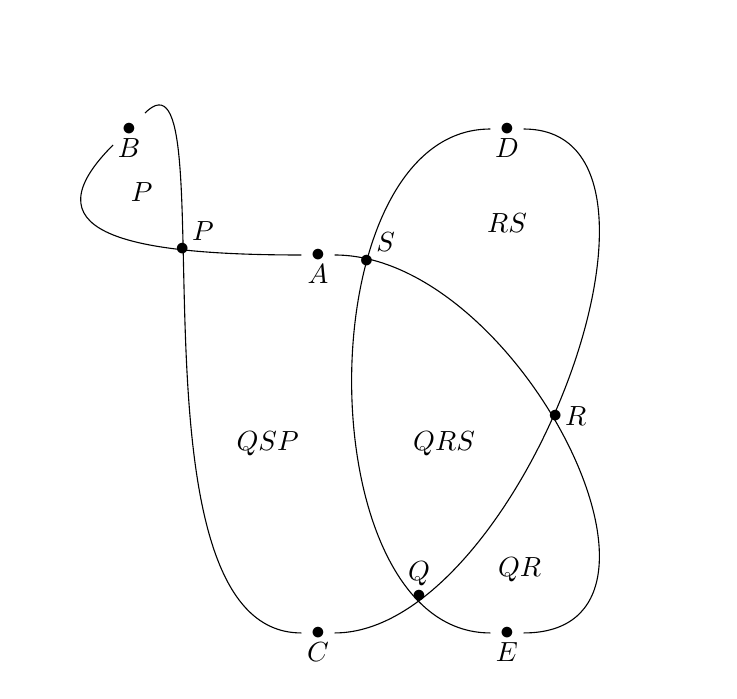
\begin{tikzpicture}[scale=8]
            \node (A) at (0.4, 0.8) {$\bullet$};
            \node (B) at (0.1, 1) {$\bullet$};
            \node (C) at (0.4, 0.2) {$\bullet$};
            \node (D) at (0.7, 1) {$\bullet$};
            \node (E) at (0.7, 0.2) {$\bullet$};
            \draw (A) node[below] {$A$} .. controls +({-1*\controlfactor}, {0*\controlfactor}) and +({-0.5*\controlfactor}, {-0.5*\controlfactor}) .. (B);
            \draw (B) node[below] {$B$} .. controls +({0.5*\controlfactor}, {0.5*\controlfactor}) and +({-1*\controlfactor}, {-0*\controlfactor}) .. (C);
            \draw (C) node[below] {$C$} .. controls +({1*\controlfactor}, {0*\controlfactor}) and +({1*\controlfactor}, {-0*\controlfactor}) .. (D);
            \draw (D) node[below] {$D$} .. controls +({-1*\controlfactor}, {0*\controlfactor}) and +({-1*\controlfactor}, {-0*\controlfactor}) .. (E);
            \draw (E) node[below] {$E$} .. controls +({1*\controlfactor}, {0*\controlfactor}) and +({1*\controlfactor}, {-0*\controlfactor}) .. (A);
            \node (P) at (0.1846, 0.808273) {$\bullet$};
            \draw (P) node[above right] {$P$};
            \node (Q) at (0.560517, 0.258828) {$\bullet$};
            \draw (Q) node[above] {$Q$};
            \node (R) at (0.776839, 0.544064) {$\bullet$};
            \draw (R) node[right] {$R$};
            \node (S) at (0.477184, 0.790679) {$\bullet$};
            \draw (S) node[above right] {$S$};
            \node (QSP) at (.32, .5) {$QSP$};
            \node (QRS) at (.6, .5) {$QRS$};
            \node (QR) at (.72, .3) {$QR$};
            \node (RS) at (.7, .85) {$RS$};
            \node (P) at (0.12, .9) {$P$};
        \end{tikzpicture}
        \caption{}
        \label{}
    \end{figure}
\newpage
\section{Finding $\eta(z)$}
    given: \\
    two borders of the shape, $A(t), B(u)$, defined as splines. \\
    the value at the borders, going up and down:
    $$\begin{aligned}
        \eta(A(t))      =& \cos(\pi t) \\
        \eta(B(u))      =& -\cos(\pi u) \\
    \end{aligned}$$
    linear interpolation:
    $$\begin{aligned}
        \eta(r\cis(\theta)) =& \eta(a(t_r))(\theta-\theta_b) + \eta(b(u_r))(\theta-\theta_a) & & \\
        \lim_{\zeta\to 0}\left(\frac{\eta(\zeta\cis\alpha)}{\zeta\cis\alpha}\right) =& 0 \\
    \end{aligned}$$
\section{intersection of a spline with a straight line}
    given a line $P + pu$ for $u \in \mathbb{R}$ and the Spline $\Lspline_{ABab}(t)$ with $t \in [0, 1]$, how many intersections are there between the two?
    $$\begin{aligned}
        P + pu =& A + at + (3B - 3A - 2a - b)t^2 + (2A - 2B + a + b)t^3 \\
        T :=& (3B - 3A - 2a - b) \\
        U :=& (2A - 2B + a + b) \\
        P_x + p_xu =& A_x + a_xt + T_xt^2 + U_xt^3 \\
        w_x :=& \frac{U_x}{U_y} \\
        (w_xP_y - P_x) + (w_xp_y - p_x)u =& (w_xA_y - A_x) + (w_xa_y - a_x)t + (w_xT_y - T_x)t^2 \\
        V_0 :=& \frac{(w_xA_y - A_x) - (w_xP_y - P_x)}{w_xp_y - p_x} \\
        V_1 :=& \frac{(w_xa_y - a_x)}{w_xp_y - p_x} \\
        V_2 :=& \frac{(w_xT_y - T_x)}{w_xp_y - p_x} \\
        u =& V_0 + V_1t + V_2t^2 \\
        P_x + p_x\left(V_0 + V_1t + V_2t^2\right) =& A_x + a_xt + T_xt^2 + U_xt^3 \\
        0 =& A_x - P_x - p_xV_0 + (a_x - p_xV_1)t + (T_x - p_xV_2)t^2 + U_xt^3 \\
        W_0 :=& \frac{A_x - P_x - p_xV_0}{U_x} \\
        W_1 :=& \frac{a_x - p_xV_1}{U_x} \\
        W_2 :=& \frac{T_x - p_xV_2}{U_x} \\
        0 =& W_0 + W_1t + W_2t^2 + t^3 \\
        e :=& \frac{-W_2}{3} \\
        f :=& e^3 + \frac{W_2W_1-3W_0}{6} \\
        g :=& \frac{W_1}{3} \\
        h :=& \sqrt{f^2 + (g - e^2)^3} \\
        t =& \sqrt[3]{f + h} + \sqrt[3]{f - h} + e \\
    \end{aligned}$$
    % example:
    % $$\begin{aligned}
    %     0 + (1+i)u =& (.15 + .9i) + -t
    %       + (3(.45 + .1i) - 3(.15 + .9i) - 2(.5 + .5i) - 1)t^2 \\
    %      &+ (2(.15 + .9i) - 2(.45 + .1i) +  (.5 + .5i) + 1)t^3 \\
    %     T :=& (3(.45 + .1i) - 3(.15 + .9i) - 2(.5 + .5i) - 1) = -1.1 - 3.4j \\
    %     U :=& (2(.15 + .9i) - 2(.45 + .1i) +  (.5 + .5i) + 1) = .9 + 2.1j \\
    %     0 + 1u =& .15 + .5t - 1.1t^2 + .9t^3 \\
    %     w_x :=& \frac{.9}{2.1} = .43 \\
    %     (.43\cdot 0 - 0) + (.43 - 1)u =& (.43\cdot .9 - .15) + (.43\cdot .5 - .5)t + (.43\cdot -1.1 - T_y)t^2 \\
    %     w_p := \frac{1}{.43 - 1} = -1.75 \\
    %     V_0 :=& ((.43\cdot.9 - .15) - (0 - 0))\cdot -1.75 = -.41 \\
    %     V_1 :=& (.43\cdot.5 - .5)\cdot -1.75 = .5 \\
    %     V_2 :=& (.43\cdot-3.4 + 1.1)\cdot -1.75 = .63 \\
    %     u =& -.41 + .5t + .63t^2 \\
    %     P_x + p_x\left(-.41 + .5t + .63t^2\right) =& A_x + a_xt + T_xt^2 + U_xt^3 \\
    %     0 =& A_x - P_x - p_x\cdot-.41 + (a_x - p_x\cdot.5)t + (T_x - p_x\cdot.63)t^2 + U_xt^3 \\
    %     W_0 :=& \frac{.15 - 0 - 1\cdot-.41}{2.1} = .63 \\
    %     W_1 :=& \frac{.5 - 1\cdot.5}{2.1} = 0 \\
    %     W_2 :=& \frac{-1.1 - 1\cdot.63}{2.1} = -1.9 \\
    %     0 =& W_0 + W_1t + W_2t^2 + t^3 = t^3 -1.9t^2 + .63 \\
    %     p :=& \frac{0+1.9^2}{3} = -1.2 \\
    %     q :=& \frac{2\cdot-1.9^3}{27} - \frac{-1.9\cdot 0}{3} + .63 = .1 \\
    %     D :=& (-1.2/3)^3 + (.1/2)^2 = -.06 \\
    %     r :=& \sqrt{-{\frac p 3}^3} = \sqrt{.4^3} = .64 \\
    %     \cos\phi =& \frac{-q}{2r} \\
    %     \phi :=& \acos\left(\frac{-q}{2r}\right) = 1.65 \\
    % \end{aligned}$$
\end{document}
